\documentclass[10pt,a4paper]{article}
\usepackage[latin1]{inputenc}
\usepackage{amsfonts}
\usepackage{amssymb}
\usepackage{listings}
\usepackage{tabularx}
\usepackage[pdftex]{graphicx}
\usepackage{url}

\lstset{tabsize=2}
\lstset{captionpos=b} %caption pos on bottom of the code
\lstset{breaklines=true}
\lstset{linewidth=\textwidth}
\lstset{basicstyle=\small\textit\ttfamily}

\author{Martin Dobiasch}
\title{midi extension for netlogo}

\begin{document}

\section{Commands of the Extension}
The prefix for all commands in the extension is "\lstinline|midi:|". 

In the documentation of the commands is always in the form \lstinline|Command Parameter|.
In a program its noted as "\lstinline|midi:Command Parameter|". The commands
are not(!) case-sensitive. 

\subsection{Midi-Commands}
\subsection{Standard Commands}
In the list below you find all standard midi commands implemented in the extension. 
Every entry is in the form ''\textit{command.name} parameters''.

Reminder: Channels are in the range 1 to 16. 
\begin{itemize}
\item \lstinline|noteon channel note volume|
\item \lstinline|noteoff channel note|
\item \lstinline|instrument channel instrument| (for a list of instruments see \cite{midi-inst})	
\item \lstinline|pitch.bend channel bend|
\item \lstinline|controller channel controller parameter|
\item \lstinline|key.pressure channel note pressure|
\item \lstinline|channel.pressure channel pressure|
\item \lstinline|volume channel volume|
\item \lstinline|expression channel expression|
\item \lstinline|modulation channel modulation|
\item \lstinline|pan channel pan|
\item \lstinline|sustain channel value|
\item \lstinline|reverb channel note volume duration|
\item \lstinline|chorus channel duration|
\item \lstinline|portamento.time channel time|
\item \lstinline|portamento channel onoff|
\item \lstinline|portamento.from channel note|
\item \lstinline|rpn channel lorpn hirpn lodata hidata|
\item \lstinline|nrpn channel lorpn hirpn lodata hidata|
\item \lstinline|reset.controllers channel|
\item \lstinline|all.notes.off channel|
\item \lstinline|pitch.sens channel semitones|
\item \lstinline|mastertune.coarse channel hidata|
\item \lstinline|mastertune.fine channel cents|
\item \lstinline|panic|
\end{itemize}

\subsubsection{The Note Command}
\lstinline|note channel note volume duration| \label{note-warning}


\begin{emph}Attention:
	This Command is a blocking-call. It plays a note with the given duration.
	After that, the program can be continued. It sets the note to the given
	channel and sleeps for the given duration. After that, it deletes the note
	from the channel. This behaviour can lead to problems when used in 
	combination with the Conductor-Utilities. 
\end{emph}

\subsection{Commands for Turtles/Agents}
\lstinline|updatepostion channel| 

This command sets a virtual position for the current turtle. The calculated
position will be set for a given channel (via parameter). Changed parameters
for the channel are pan and expression. Base point for the calculation of the
values is the origin of the coordinate system of the NetLogo-Model. The values
are scaled according to the maximum on the coordinate axis. 

%Dieser Befehl setzt eine eine Position im akustischen Raum f"ur die aktuelle
%Turtle, kann also nur in einem Turtle-Context angewandt werden. Die Position
%wird f"ur die Turtle die den Befehl aufruft errechnet und dann als virtuelle
%Position auf den "ubergebenen Channel gelegt (siehe auch \ref{sec:sheet-channel}. 
%Ver"andert werden die Parameter Pan und Expression. Ausgangspunkt f"ur die
%Berechnung ist der Koordinaten-Ursprung des NetLogo-Models. Als maximaler Wert
%f"ur die Skalierung wird auch jeweils der maximale Wert des Koordinatensystems
%verwendet wird. Das hei"st wenn das Model zB. auf der positiven X-Achse mehr Werte
%zul"asst als auf der negativen. Ist die Abstufung auf der positiven Seite feiner.

\subsection{Commands for the Condcutor}
\subsubsection{clear.sheets}
Syntax: \lstinline|conductor.clear.sheets|

Clears all known sheets. 
\subsubsection{add.to.sheet}
Syntax: \lstinline|conductor.add.to.sheet sheet time.distance command|

This command adds a command to the end of a sheet (given by the parameter). The command
will be executed after the interval given by the parameter \lstinline|time.distance| (in ms).
This is also the interval used for further calculation of starting points of following commands.

Example: 
%Dieser Befehl f"ugt dem angegebenen Notenblatt am Ende ein Kommando hinzu. Das
%Kommando wird nach Ablauf der durch \lstinline|time.distance| angegebenen Zeit
%(in ms) ausgef"uhrt. Zus"atzlich ist das der Zeitpunkt von welchem aus der 
%Zeitpunkt f"ur ein m"ogliches nachfolgendes Kommando berechnet wird. Beispiel:
\begin{lstlisting}[language=Logo]
midi:conductor.clear.sheets
midi:conductor.add.to.sheet 1 10 "midi:noteon 2 60 1"
midi:conductor.add.to.sheet 1 2000 "midi:noteoff 2 60"
midi:conductor.start
\end{lstlisting}

After 10ms, Sheet 1 will play the note ''60'' (volume = 1) on Channel 2. Two seconds
after that, it will clear-remove the note from the channel. 

%Nach Ablauf von zehn Milisekunden wird vom Notenblatt Eins auf dem Midi-Kanal
%Zwei die Note mit dem Wert 60 gespielt. Nach zwei Sekunden, also nach insgesamt
%2010 Milisekunden verstummt die Note wieder. 

\subsubsection{add.to.sheet.list}
Syntax: \lstinline|conductor.add.to.sheet.list sheet command.list|

This command adds command of the list ''command.list'' to the end of the given
sheet. Commands in the list have to take the form \lstinline|[time.code command]|
The time-codes work analogous to the time-codes of \lstinline|add.to.sheet|. The added
commands have to be strings. (This is due to the lack of possibility of having
commands as parameters at the time of development in July/October 2010), therefore the
commands should be checked for syntax. Otherwise there will be a lot of exceptions raised
during runtime. 
One advantage of this command is that, with a view modifications the output from 
''to logo''-Command of the MidiCSD-Toolkit for Office \cite{MidiCSD} by Dr. Erich Neuwirth
can be used. 
See the example below: 

%Dieses Kommando f"ugt dem angegebenen Notenblatt am Ende die Kommandos aus der 
%Liste ein. Die Kommando-Liste hat eine einfache Syntax: \lstinline|[time.code command]|
%Die Time-Codes funktionieren analog zu denen des \lstinline|add.to.sheet| Befehls.
%Das Kommando muss aber als String angegeben werden! Das kommt daher, dass NetLogo
%zum Entwicklungszeitpunkt (Juli-Oktober 2010) nicht ausreichend mit dem Syntax-Typ
%''Command'' umgehen konnte. Die Befehle sollten also getestet werden bevor sie
%auf die Notenbl"atter geschrieben werden. Der Vorteil dieses Befehls ist, dass
%er, mit geringen Modifikationen, die Ausgabe des ''to Logo'' des MidiCSD-Toolkits \cite{MidiCSD}
%f"ur Office Dr. Erich Neuwirth verwendet kann. Das untenstehende Beispiel demonstriert,
%wie der Befehl eingesetzt werden kann. 
\begin{lstlisting}[language=Logo]
to test
  clear-all
  midi:conductor.clear.sheets
 
  midi:conductor.add.to.sheet.list 1 [
		[0 "midi:note 10 45 1 200"]
		[200 "midi:note 10 45 0.7 200"]
		[200 "midi:note 10 45 0.7 200"]
		[200 "midi:note 10 45 0.7 200"]
		[200 "midi:note 10 45 1 200"]
  ]
  midi:conductor.add.to.sheet.list 2 [
		[200 "midi:pan 10 -0.75"]
		[200 "midi:pan 10 -0.5"]
		[200 "midi:pan 10 -0.25"]
		[200 "midi:pan 10 0"]
  ]
  
  midi:conductor.add.to.sheet.list 3 [
		[5 "midi:expression 10 0.75"]
		[200 "midi:expression 10 0.69"]
		[200 "midi:expression 10 0.63"]
		[200 "midi:expression 10 0.56"]
		[200 "midi:expression 10 0.5"]
  ]
  
  midi:conductor.setplaymode.endless

  midi:conductor.start
end
\end{lstlisting}

\subsubsection{restart}
Syntax: \lstinline|conductor.restart|

The conductor will set the pointer to the commands to be executed to the beginning. 
%Die Position auf den Notenbl"attern wird wieder auf Null gesetzt. Alle Notenbl"atter
%werden also wieder von Vorne abgearbeitet. 
\subsubsection{conduct}
Syntax: \lstinline|conductor.conduct|

The conductor is asked to execute all commands which are due at the moment of the call.
%Der Dirigent wird angewiesen die aktuell anfallenden Befehle auf den Notenbl"attern
%abzuarbeiten. 

\subsubsection{setplaymode.endless}
Syntax: \lstinline|conductor.setplaymode.endless|

The conductor has different play modes. When the play mode is set to endless,
every time a sheet is finished it will start from the beginning. Expressed
differently sheets aren't linear in this mode, they are circular. 
Attention: The play mode doesn't respect different lengths of sheets. The 
execution is not synchronized. A sheet starts from its beginning as soon as it
reaches the end, with no respect to other sheets. 
%Erreicht ein ''Musiker'' auf seinem Notenblatt das Ende, soll er wieder von 
%Vorne beginnen. Anders gesagt: Die Notenbl"atter sind nun nicht mehr linear
%sondern Kreise. Auf unterschiedliche L"angen/Dauer der Notenbl"atter wird aber
%nicht geachtet. 

\subsubsection{setplaymode.normal}
Syntax: \lstinline|conductor.setplaymode.normal|

In this play mode the conductor doesn't restart a sheet when its finished. 
%Anders als beim Endlos-Playmode wird der Dirigent angewiesen, wenn ein Notenblatt
%zu Ende ist, nicht wieder von Vorne zu beginnen sondern aufzuh"oren. 
\subsubsection{start}
Syntax: \lstinline|conductor.start|

This command starts the ConductorThread ie. The Conductor is asked to start
conduction in the background. The execution of the program continues as soon
as the thread is started. 
%Dieser Befehl wei"st den Dirigenten an im Hintergrund zu dirigieren. Das Programm
%l"auft weiter w"ahrend im Hintergrund die Notenbl"atter abgearbeitet werden. 
(Siehe auch \lstinline|conductor.stop|)
\subsubsection{stop}
Syntax: \lstinline|conductor.stop|

This command stops the ConductorThread ie. The conductor is asked to end 
conduction (done in the background). 
%Dieser Befehl weist den Dirigenten an seine Arbeit zu beenden. Die Abarbeitung
%der Notenbl"atter im Hintergrund wird beendet. 


\section{The Conductor in Midi-NetLogo}
The Conductor offers the chance to define sequences which can be executed independently of each other.
These sequences can contain any command available in NetLogo. 

This can be used for teaching of threads in informatics classes. A thread is not
different from a Sheet.  

\subsection{Concept}
As the name suggests the extension uses the metaphor of an orchestra. The conductor has 
control of multiple musicians who execute some actions. He/she decides when the
orchestra should start playing and when to stop. Also the orchestra can be asked to
start again from the beginning. 

Every program needs some scheduling mechanism for its threads. The conductor is doing
this job in the extension. 

\subsection{About the implementation}
As mentioned above NetLogo is extended trough a central instance called the Conductor. 
It has the following features: \begin{itemize}
\item delete all sheets
\item add something to a sheet
\item add something to a sheet with a time-code
\item set everything to start
\item condcut
\item play endless / in a loop or play normal. 
\end{itemize}

\subsubsection{Sheets - Channels}\label{sec:sheet-channel}
The Conductor holds a fixed amount of 16 sheets because midi has 16 channels.
These midi-channels are numbered 1 - 16, where the sheets have indices/numbers 0 - 15.
This problem can be solved with a variable for the agents, assigning a channel to every agent (
where the id of the agent is the index of the sheet)

\begin{lstlisting}[language=Logo]
turtles-own [channel]
...
to init
  set channel who + 1
end

...

to some.procedure
	ask turtles[
		midi:instrument channel 60
	]
end
\end{lstlisting}


\subsubsection{Events}
The central purpose of the Sheets is to execute commands in some chronological order. 
There are two possible ways to add commands to a sheet. 
\begin{itemize}
\item conductor.add.to.sheet
\item conductor.add.to.sheet.list
\end{itemize}
Both commands act mostly the same. However, the second needs a list of timestamped commands.
The first one adds only one command.

\begin{itemize}
\item conductor.add.to.sheet
\item conductor.add.to.sheet.list
\end{itemize}

\section{Technical Details of the implementation}
\subsection{Structure}
\begin{figure}[hbt]
	\centering
		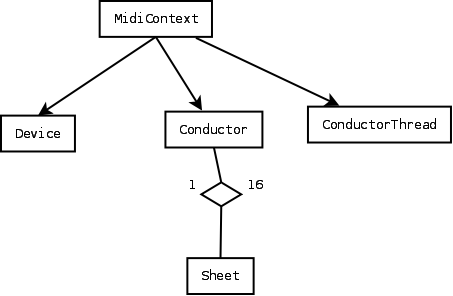
\includegraphics[scale=0.3]{germanDoc/fig/struktur.png}
	\caption{Struktur}
	\label{fig:struktur}
\end{figure}

The extension is based on a simple structure. When the extension is loaded an instance
of \lstinline|MidiContext| is created. This instance provides access to the midi-device
and the \lstinline|Contductor|. For synchronizing issues there is a semaphor-like mechanism
for managing the access to the objects. 

\textit{Issues may arise since I only used bool types for managing request and no
counters. However, I do not expect any significant problems since there is only one object to
take care of and only one NetLogo-Instance. The implementation can be found in ''MidiContext.java''}

\subsection{MidiContext}
It takes care of the synchronisation of the threads accessing the midi-device.
(Only one device will be opened.) To send a command to the device, the caller
has to reserve the device by calling \lstinline|MidiManager.getMidiContext().getDevice()|
When the device is not needed it should be marked as free again by calling 
\lstinline|MidiManager.getMidiContext().releaseDevice()|.  

\subsection{Conductor}
The Context contains an instance of the Conductor. This class should help
the user by creating a virtual conductor. Therefore there will be up to 16 sheets (since midi only has
16 channels). The access to the conductor is also synchronized with 
\lstinline|MidiManager.getMidiContext().getConductor();|
and \lstinline|MidiManager.getMidiContext().releaseConductor();|

\subsection{Sheet}
This class should help managing commands, which should be executed with a specific time-code.
(Sheets are the pendant to streams in MidiCSD \cite{MidiCSD})
Each sheet has a list of commands, which can be any NetLogo-command. The commands are only
stored and passed to the interpreter on the fly. While this is poses a drawback to the running time, it also
increases flexibility. Thus virtual musicians (turtles) can not only play music, they can also
walk. 
In the source-code you can also find an implementation for a ''Midi-Engine'', which restricts the
sheets to a few midi-based commands that are rendered to a stream. 


\subsection{ConductorThread}
In order to allow the user to hide the work of the Conductor in the background, 
there is the ConductorThread. Once started, it works through the sheets piecewise
At each step it reserves access to the conductor to get the scheduled
Commands. After the execution of the commands, the thread sleeps for 100ms so as not to
block the entire system. 

\subsection{New Commands}
In order to implement new midi-commands, there is a class \lstinline|MidiCommand|. It has
two methods: \lstinline|preAction| und \lstinline|postAction|. Every new
Midi-Command, if derived from MidiCommand, can get access to the mididevice by simply
calling \lstinline|preAction| and release the lock of the device by calling \lstinline|postAction|
Thus, the flexibility of the code is increased and changes to the code for opening the
midi-device have to be performed only once. 

\addcontentsline{toc}{section}{References}
\bibliographystyle{amsplain} %take natbib if you need refernces by Author&year
\bibliography{germanDoc/lit}

\end{document}


